\documentclass[11pt]{article}
\usepackage[margin=0.9in]{geometry}
\usepackage{amsmath,amssymb}
\usepackage{booktabs}
\usepackage{graphicx}
\usepackage{microtype}
\usepackage[hidelinks]{hyperref}
\usepackage{float}

\title{\bfseries Composite versus Direct: the problems, and what the numbers say}
\date{}
\author{}

\begin{document}
\maketitle
\vspace{-3em}

\section{The setup}

Every problem has the form
\[
f(x) \;=\; g\bigl(h(x)\bigr), \qquad x \in [0,1]^6 ,
\]
with $h$ the \emph{intermediate} (expensive, unknown) and $g$ the \emph{outer
map} (cheap, known in closed form). Two surrogates compete:

\begin{center}
\begin{tabular}{llll}
\toprule
 & Observes & Models & Predicts $f$ by \\
\midrule
\textbf{Direct} & $f(x_i)$ only & a GP on $f$ & reading off that GP \\
\textbf{Composite} & $h(x_i)$ & a GP on each $h_j$ & sampling $h$ and applying $g$ \\
\bottomrule
\end{tabular}
\end{center}

\noindent Both get the same inputs, the same budget, the same initial design
and the same acquisition function. Only the surrogate differs.

\subsection{The intermediates}

$h$ is not an analytic test function. It is a draw from the \emph{same}
Gaussian process family the surrogates assume, built from random Fourier
features:
\[
h(x)=\sqrt{\tfrac{2}{M}}\sum_{m=1}^{M} a_m\cos(\omega_m^\top x + b_m),
\qquad a_m\sim\mathcal N(0,1),\ b_m\sim U(0,2\pi),\ \omega_m\sim\mathcal N(0,\ell^{-2}I),
\]
with $M=1024$ and $\ell=0.5$, then standardised so it has mean $0$ and
standard deviation $1$.

This matters for the comparison. If $h$ were something like Rastrigin,
Composite might win or lose because a GP happens to model \emph{that function}
well or badly, and we would learn nothing about $g$. Drawing $h$ from the
surrogate's own prior removes that: Composite's model of $h$ is correct by
construction, so every remaining difference is attributable to the outer map.

Standardising also puts the mean at zero, so $h$ takes both signs. Without
that, $h^2$ would be injective over the region actually visited and the whole
information question would be empty.

\paragraph{Range.} Over $[0,1]^6$, $h$ reaches about $[-4.3,+3.8]$: sd exactly
$1$, with $5\%$ of the domain beyond $|h|>2$ and $0.3\%$ beyond $|h|>3$. The
range saturates --- sampling a million points finds no more than sampling ten
thousand --- because it is a property of the function, not of the sampling.
That is why root placements at $\pm2$ sit inside the bulk while a vertex at
$h=3$ sits at the edge of what is reachable.

\paragraph{Several intermediates.} When $k>1$, each $h_j$ is an independent
draw with its own seed ($1000\times\text{draw} + j$); measured correlation
between them is $-0.10$, i.e.\ zero. Maps sharing a draw seed share the same
$h_1$, so switching $g$ never changes the underlying functions.

\begin{table}[htbp]
\centering
\footnotesize
\setlength{\tabcolsep}{4pt}
\caption{Every problem. $k$ is the number of intermediates, $\bar n$ the
measured average number of $h$ values consistent with one observation, and
the last column what $g$ throws away. A dash in $\bar n$ means the fiber is
continuous, so the count is infinite.}
\label{tab:problems}
\begin{tabular}{@{}l c l c l l@{}}
\toprule
Problem & $k$ & $g(h)$ & $\bar n$ & Bijective? & What $g$ discards \\
\midrule
\texttt{identity} & 1 & $h$ & 1.00 & \textbf{yes} & nothing \\
\texttt{exp\_b1} & 1 & $e^{h}$ & 1.00 & \textbf{yes} & nothing (monotone, positive) \\
\texttt{sinh\_b1} & 1 & $\sinh h$ & 1.00 & \textbf{yes} & nothing (monotone, unbounded) \\
\texttt{shiftsq\_c3} & 1 & $(h-3)^2$ & 1.01 & \textbf{yes} & sign of h - c \\
\midrule
\texttt{shiftsq\_c0} & 1 & $h^2$ & 2.00 & no & sign of h - c \\
\texttt{shiftsq\_c0.5} & 1 & $(h-0.5)^2$ & 2.00 & no & sign of h - c \\
\texttt{shiftsq\_c1} & 1 & $(h-1)^2$ & 1.95 & no & sign of h - c \\
\texttt{shiftsq\_c2} & 1 & $(h-2)^2$ & 1.37 & no & sign of h - c \\
\texttt{abs} & 1 & $|h|$ & 2.00 & no & sign of h (with a kink) \\
\texttt{cos\_w1} & 1 & $\cos h$ & 2.03 & no & which of many preimages \\
\texttt{cos\_w2} & 1 & $\cos 2h$ & 5.04 & no & which of many preimages \\
\texttt{relu} & 1 & $-\max(h,0)$ & $\boldsymbol{\infty}$ & no & everything below zero (censoring, away from the optimum) \\
\texttt{clip\_c2} & 2 & $\mathrm{clip}(2h_1,-1,1)+h_2$ & --- & no & the clipped coordinate inside the saturated regions \\
\texttt{sum} & 2 & $h_1+h_2$ & --- & no & how the sum splits (Truss / RCM40) \\
\texttt{product} & 2 & $h_1h_2$ & --- & no & how the product factors, and sign (DTLZ2) \\
\texttt{norm} & 2 & $\sqrt{h_1^2+h_2^2}$ & --- & no & direction (Color) \\
\texttt{max} & 2 & $\max(h_1,h_2)$ & --- & no & the smaller value (Lake) \\
\texttt{ratio} & 2 & $\frac{\sigma(h_1)}{0.05+\sigma(h_1)+\sigma(h_2)}$ & --- & no & scale (RGB) \\
\bottomrule
\end{tabular}
\end{table}


\section{What $\bar n$ means}

$\bar n$ is the average number of $h$ values that could have produced the $y$
you observed:
\[
\bar n=\mathbb E\bigl[\,|g^{-1}(y)|\,\bigr].
\]
$\bar n=1$ means $y$ determines $h$ --- the map is injective, and observing
$h$ tells you nothing new. $\bar n = 2$ means a typical observation leaves two
candidates.

It is \emph{measured}, by counting crossings of $g(z)-y$ over the range $h$
actually reaches, not inferred from the algebra. The two come apart:
\texttt{shiftsq\_c3} is a parabola, and so two-to-one on paper, but its vertex
sits at $h=3$ where $h$ almost never goes, so in practice $\bar n=1.01$ and it
behaves as a bijection.

The same measurement needs care with flat regions. $-\max(h,0)$ sends the
entire half-line $h\le0$ --- about half the domain --- to a single value, so
those observations have an \emph{infinite} preimage set. A crossing counter
reports $1$ there, because a flat region never crosses. \texttt{relu} is
therefore marked $\infty$ and grouped with the non-bijective maps.

\section{Results}

\begin{table}[H]
\centering
\small
\caption{Bijective maps: final $\log_{10}$ regret over 20 runs, mean $\pm$ SD. Gain is Direct $-$ Composite, so positive favours Composite. $p$ is a one-sided paired $t$-test.}
\label{tab:bij}
\begin{tabular}{l r r r r}
\toprule
Problem & Direct & Composite & Gain & $p$ \\
\midrule
\texttt{identity} & $-1.789\pm1.323$ & $-2.198\pm1.176$ & $+0.409\pm1.138$ & 0.062 \\
\texttt{exp\_b1} & $-2.868\pm0.378$ & $-3.493\pm1.474$ & $+0.625\pm1.309$ & 0.023 \\
\texttt{sinh\_b1} & $-0.490\pm1.133$ & $-0.933\pm1.105$ & $+0.444\pm1.126$ & 0.047 \\
\texttt{shiftsq\_c3} & $-4.824\pm1.282$ & $-6.571\pm1.762$ & $+1.747\pm1.482$ & $<$0.001 \\
\bottomrule
\end{tabular}
\end{table}

\begin{table}[H]
\centering
\small
\caption{Non-bijective maps, same convention.}
\label{tab:nonbij}
\begin{tabular}{l r r r r}
\toprule
Problem & Direct & Composite & Gain & $p$ \\
\midrule
\texttt{shiftsq\_c0} & $-5.650\pm1.306$ & $-7.665\pm0.580$ & $+2.015\pm1.454$ & $<$0.001 \\
\texttt{shiftsq\_c0.5} & $-5.510\pm1.134$ & $-7.824\pm0.284$ & $+2.313\pm1.041$ & $<$0.001 \\
\texttt{shiftsq\_c1} & $-5.594\pm1.191$ & $-7.797\pm0.445$ & $+2.203\pm1.181$ & $<$0.001 \\
\texttt{shiftsq\_c2} & $-5.494\pm0.899$ & $-7.927\pm0.133$ & $+2.433\pm0.893$ & $<$0.001 \\
\texttt{abs} & $-2.746\pm0.575$ & $-3.093\pm0.582$ & $+0.347\pm0.762$ & 0.028 \\
\texttt{cos\_w1} & $-4.429\pm2.566$ & $-6.497\pm1.863$ & $+2.068\pm2.497$ & $<$0.001 \\
\texttt{cos\_w2} & $-4.647\pm0.907$ & $-6.820\pm0.804$ & $+2.173\pm1.166$ & $<$0.001 \\
\texttt{relu} & $-1.303\pm1.150$ & $-1.847\pm1.283$ & $+0.545\pm1.600$ & 0.072 \\
\texttt{clip\_c2} & $-1.166\pm0.491$ & $-2.964\pm2.285$ & $+1.798\pm2.103$ & $<$0.001 \\
\texttt{sum} & $-1.884\pm1.208$ & $-2.230\pm1.128$ & $+0.346\pm1.149$ & 0.097 \\
\texttt{product} & $-1.167\pm1.125$ & $-1.378\pm1.082$ & $+0.211\pm1.109$ & 0.203 \\
\texttt{norm} & $-1.885\pm0.355$ & $-2.174\pm0.218$ & $+0.290\pm0.276$ & $<$0.001 \\
\texttt{max} & $-1.092\pm0.507$ & $-1.706\pm0.626$ & $+0.615\pm0.725$ & $<$0.001 \\
\texttt{ratio} & $-2.172\pm1.120$ & $-2.280\pm1.364$ & $+0.109\pm0.820$ & 0.280 \\
\bottomrule
\end{tabular}
\end{table}


\subsection{How to read these}

\paragraph{The metric.} Simple regret, $R_T=f_{\text{best}}(T)-f^\star$, after
$T=45$ evaluations, reported as $\log_{10}R_T$. Lower is better. Because it is
a log, the \emph{gain} is a ratio: a gain of $+2$ means Composite's final
regret is $100$ times smaller.

\paragraph{The spread.} Quoted as $\pm$ one standard deviation across the $20$
runs, not a standard error --- it describes how much a single run varies, not
how precisely the mean is known. The standard error is roughly $1/\sqrt{20}$
of it.

\paragraph{The $p$-value.} A one-sided paired $t$-test, asking whether
Composite's mean regret is lower. Paired because both arms share an initial
design within each run, so the comparison is run by run and the large
variation between designs cancels.

\paragraph{A caution.} These distributions are skewed --- several standard
deviations exceed their own means --- so a $t$-test can be carried by a few
large wins. On \texttt{relu}, Composite actually loses $11$ of $20$ runs while
still posting a positive mean gain. A $p$-value near $0.05$ on a row with a
large SD should be read as suggestive rather than settled.

\paragraph{The $-8$ floor.} $\log_{10}$ regret is clamped at $-8$. Four
\texttt{shiftsq} rows have Composite at $-7.7$ to $-7.9$, so they are pressed
against it and their gains are lower bounds. The reference optimum is known to
about $10^{-15}$, so the clamp is discarding real resolution and should be
lowered.

\section{Convergence}

\begin{figure}[H]
\centering
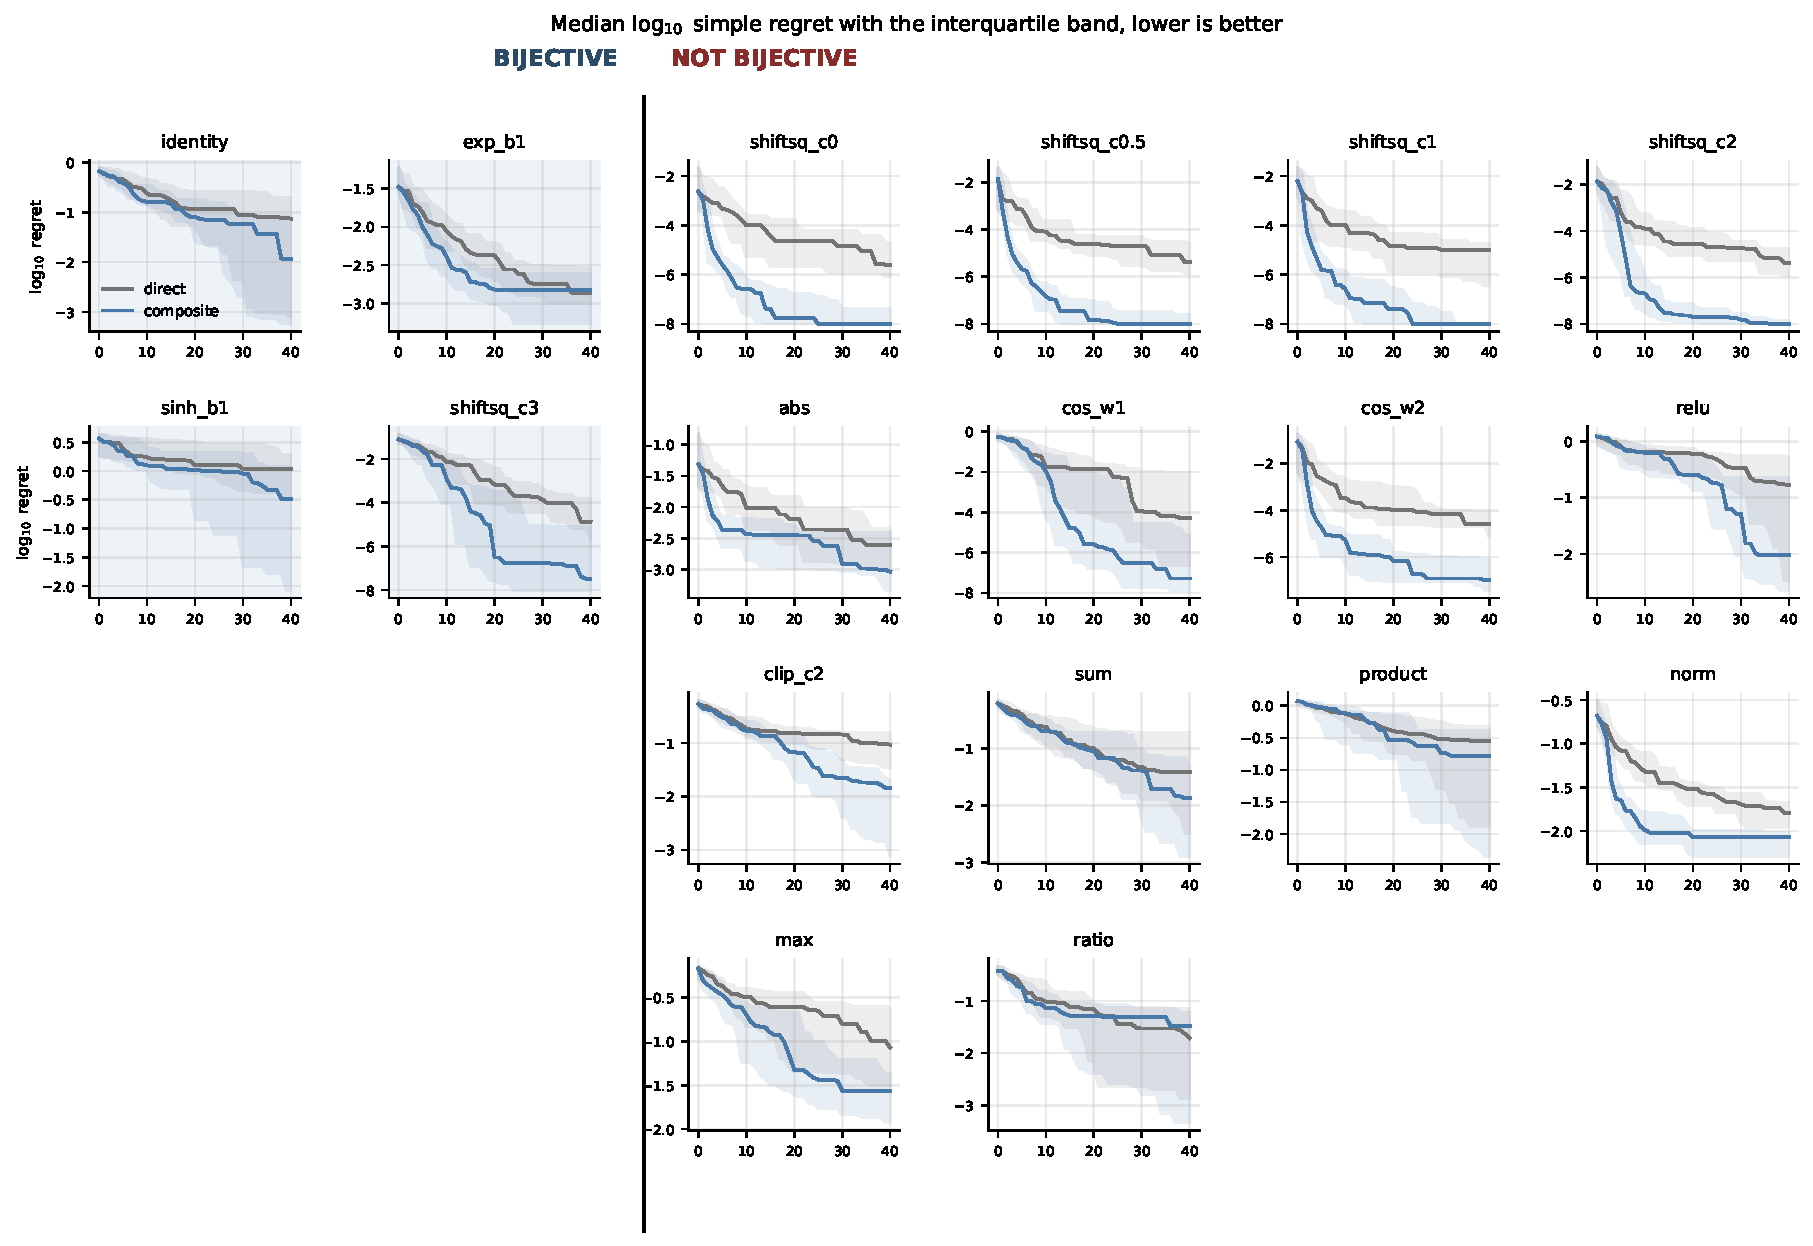
\includegraphics[width=\linewidth]{../figures/bo_curves.pdf}
\caption{Median $\log_{10}$ regret against evaluation, interquartile band
shaded. Bijective maps left of the rule, non-bijective right. Composite wins
throughout \emph{both} sides, which is the central observation: the advantage
is not information, because on the left there is none to be had.}
\end{figure}

\section{Why Direct loses even when nothing is hidden: $z^3$}

\texttt{mono3}, $g(h)=h^3$, is strictly increasing. It is bijective, so
observing $h$ conveys nothing that $y$ does not already determine. Composite
should have no advantage --- and it has a large one. A plain regression
experiment, with no optimisation anywhere, shows why.

Eighty training points, twenty held out, $30$ fits per map. RMSE is divided by
the standard deviation of whatever is being predicted, so $1.0$ means no
better than guessing the mean.

\begin{table}[H]
\centering\small
\caption{Held-out RMSE, normalised. ``Fitted'' means both models estimate
their hyperparameters by maximum likelihood, so neither is given anything the
other lacks.}
\begin{tabular}{l r r r}
\toprule
 & Direct & \multicolumn{2}{c}{Composite (fitted)} \\
\cmidrule(lr){3-4}
Problem & on $f$ & on $h$ (inner) & on $f$ (outer) \\
\midrule
\texttt{identity} & $0.588$ & $0.588$ & $0.588$ \\
\texttt{mono3} $=h^3$ & $\mathbf{1.071}$ & $0.588$ & $\mathbf{0.817}$ \\
\texttt{root3} & $1.287$ & $0.588$ & $0.962$ \\
\texttt{shiftsq\_c0} $=h^2$ & $1.056$ & $0.588$ & $0.865$ \\
\bottomrule
\end{tabular}
\end{table}

Three things to read off it.

\paragraph{The inner RMSE is the same in every row, $0.588$.} It must be: $h$
is literally the same function in all four, and Composite always fits the same
GP to it. A useful check that nothing else is varying.

\paragraph{Direct scores above $1.0$ on all three nonlinear maps.} It is worse
than predicting the mean of $f$. With eighty training points, a stationary GP
placed on $h^3$ has negative skill.

\paragraph{Composite, on the same eighty points with the same fitted
hyperparameters, scores $0.817$.} Nothing is being hidden from Direct: $h^3$ is
bijective, so $y$ determines $h$ exactly. Both models estimate their own
kernel. The only difference is that one models $h$ and applies the known cube
afterwards.

So Direct's failure is not a shortage of data and not a worse fit. It is that
$f=g(h)$ is \emph{not a Gaussian process} when $g$ is nonlinear, and a GP
placed directly on $f$ is the wrong shape of model. That is misspecification,
isolated from information, in one table.

\texttt{identity} is the control: $0.588$ against $0.588$, identical to three
figures, because there $f=h$ and the two models are the same model.

\section{What this means overall}

\begin{itemize}\itemsep2pt
\item \textbf{Composite wins on nearly every problem}, bijective or not,
usually by one to two orders of magnitude in final regret.
\item \textbf{Bijectivity does not predict the gain.} \texttt{shiftsq\_c3} is
effectively bijective and gains $+1.75$; \texttt{abs} is two-to-one and gains
$+0.35$. The two groups overlap heavily.
\item \textbf{The reason is that most of the advantage is not information.}
When $g$ is nonlinear, $f$ is not a GP and Direct is fitting the wrong model.
Bijectivity removes the information channel and leaves that one untouched.
\item \textbf{The quantity that does track the gain is how low the problem can
be driven at all} ($r=-0.93$ against Composite's final regret). Where $g$ is
flat at its optimum there is a broad near-optimal plateau and the gap can be
enormous; where $g$ is steep there, neither arm gets far and the gap is small.
\end{itemize}

\paragraph{Left out.} \texttt{cos\_w4} is excluded pending a closer look. It
has the most preimages of any map ($\bar n=9.75$) and nearly the smallest gain,
because at $\omega=4$ the posterior uncertainty in $h$ spans most of a
half-period and Composite's predictive on $f$ becomes as wide as $f$ itself ---
it knows $h$ and that tells it nothing about the objective.

\paragraph{One caveat on these tables.} Composite here is given the
generator's true kernel, while Direct must estimate one. On \texttt{identity},
where no misspecification is possible, that alone is worth the entire $+0.409$
gain; making Composite fit its hyperparameters drops it to $+0.206$. The
nonlinear rows keep their large gains either way, but the bijective rows
should be read as upper bounds until the all-fitted grid is run.

\end{document}
